\section{Linked Data Query Optimization Framework}
\label{sec:framework}
Existing ad-hoc strategies for selecting Linked Data sources have shown to improve the performance of Linked Data query processing. However, there exists no optimization technique that goes beyond source selection to consider the entire process of Linked Data querying. Here, we provide a systematic study of existing Linked Data querying approaches~\cite{hartig_executing_2009,harth_data_2010,ladwig_linked_2010} to model the querying process in terms of operators of a query plan. The goal is to provide the first \emph{systematic solution towards Linked Data query optimization}, which considers the effect of query operators to compute and guarantee the (Pareto-)optimality of query plans. 

%For optimizing Linked Data queries, we systematically captures all operators needed, incorporate them into a query plan, and briefly, discuss how to estimate their impacts on the optimization objectives cost and outputs. 

\subsection{Query Operators}
\label{sec:ops}
%For processing linked data queries, sources containing data for query triple patterns have to be retrieved (possibly from remote sources). We use a \emph{source scan} operator to represent sources. Then, standard query operators are adopted to process triples retrieved from these sources.
%Triples in the same source however, can be used to answer different patterns. Selecting triples from sources is captured by the \emph{selection} operator. Triples for a pattern retrieved from all sources are then combined via the \emph{union} operator, and finally, combined with triples retrieved for other patterns via \emph{join}: 
% when these patterns share a common variable, via union otherwise. 
The standard query operators table scan, selection, union and join are adopted to model the Linked Data querying process. The main difference to traditional query processing is that the availability of data indexes cannot be assumed in the general case. Only some basic statistics about sources can be assumed to be available such that given a triple pattern, relevant sources can be determined~\cite{harth_data_2010,ladwig_linked_2010}. However, entire sources have to be retrieved. This is conceptually similar to a table scan. The difference is that often, sources have to be retrieved from remote sites via HTTP URI lookup. Moreover, several sources may contain answers for one single query predicate (triple pattern), and vice versa, one single source source may be used for several predicates.  

\begin{definition}[Source Scan] The input of a source scan operator $scan_d$ is the source URI $d$.
% consists of the data contained in
%such a source. 
Executing this operator outputs all triples in $d$, i.e. $scan_d = T^d$.
\end{definition}

\begin{definition}[Selection]  A selection $\sigma_{T^d}(t)$ is performed on the input $T^d$ to output
triples in $T^d$ that match triple pattern $t$, i.e. $\sigma_{T^d}(t) = \mu_{T^d}(t)$. 
\end{definition}

Two triple patterns $t_i$ and $t_j$ (their outputs to be more precise) that share a common variable are combined through a standard join operator $t_i\Join t_j$. In general, $T_i\Join T_j$ joins any subexpression $T_i \subset Q$ with one other $T_j \subset Q$. 

\begin{definition}[Union] As usual, $\bigcup(I_1,\ldots,I_n)$
outputs the union of its inputs $I_i$, $1\leq i \leq n$, where every input $I_i$ may stand for results for one triple pattern, $I_i = \mu(t)$, or subexpression, e.g. $I_i = \mu(T)$. Because a triple pattern can match several sources, $I_i$ may also capture partial results for a pattern $t$ such that the union
$\bigcup(\sigma_{T^{d_1}}(t),\ldots,\sigma_{T^{d_n}}(t))$ combines results from several selection operators.   
\end{definition}

For clarity of presentation, we assume query triple patterns form a connected graph such that join is the only operator used to combine triples from different patterns. 


\subsection{Query Plan}
\label{sec:basicshape}
Query plans for relational databases generally consist of access plans
for individual relations whose outputs are then processed by join and
other operators. We take a similar approach and create an
access plan for each triple pattern, which consists of source scan, selection and union
operators:

\begin{definition}[Access Plan]
  Given a query $Q$, let $t \in Q$ be a triple pattern in $Q$ and $D =
  source(t)$ be the set of sources for $t$. An \emph{access plan}
  $p(t)$ for $t$ is a tree-structured query plan constructed in the
  following way: 1) At the lowest level, the leaf nodes of $p(t)$ are
  source scan operators, one $scan_{d_i} = T^{d_i}$ for each $d_i \in
  D$; 2) the next level contains selection operators, one for
  processing the output of every scan operator, i.e. we have
  $\sigma_{T^{d_i}}(t)$ for every $d_i \in D$; 3) the root node is a
  union operator
  $\bigcup_t(\sigma_{T^{d_1}}(t),\ldots,\sigma_{T^{d_{|D|}}}(t))$ that
  combines the outputs of all selection operators for $t$.

  % \begin{itemize}
  % \item At the lowest level, the leaf nodes of $p(t)$ are source scan
  %   operators, one $scan_{d_i} = T^{d_i}$ for each $d_i \in D$.
  % \item The next level contains selection operators, one for
  %   processing the output of every scan operator, i.e. we have
  %   $\sigma_{T^{d_i}}(t)$ for every $d_i \in D$.
  % \item The root node is a union operator
  %   $\bigcup_t(\sigma_{T^{d_1}}(t),\ldots,\sigma_{T^{d_{|D|}}}(t))$
  %   that combines the outputs of all selection operators for $t$.
  % \end{itemize}
\end{definition}

At the next levels, the outputs of access plans' root operators are
successively joined to process all triple patterns of the query,
resulting in a \emph{tree of operators}. However, in Linked Data query
processing, it is often the case that a single Linked Data source
contains data matching several triple patterns. It is therefore
possible that a data source is used for more than one query triple
pattern. In this case it is detrimental to execute the scan operator
more than once as this will incur network costs that can be
avoided. We therefore perform \emph{operator sharing}, where the
output of a source scan operator is used as input for more than one
selection operator, i.e. the output is shared. This means that access
plans may overlap and the query plan is no longer a tree, but
has the form of a directed acyclic graph (DAG) \cite{Neumann_2005}.

In a DAG-shaped plan the outputs of shared operators are read multiple
times, which is not possible if the data is only passed between
operators. There are several possible strategies for executing
DAG-shaped plans \cite{Neumann_2005}. One strategy is to store the
outputs of shared operators in temporary buffers (on disk or in
memory), from which subsequent reads are served. This strategy incurs
the often not inconsiderable overhead for writing and storing the
temporary buffer. A different strategy uses a push-based execution
mode, where operators push their output to subsequent operators in the
DAG, resulting in a reversed control flow (compared to the classic
iterator model). Instead of having several operators consuming their
shared input independently, any output of a shared operator is
processed by its consumers at the same time. This push-based execution
(using symmetric hash join) was employed in previous work on Linked
Data query processing \cite{ladwig_linked_2010,sihjoin_2011} and is
also used in our implementation.

%\begin{definition}[Linked Data Query Plan]
%  Given the query $Q=\{t_1,\ldots,t_n\}$ and the corresponding access plans for every triple pattern $A(Q) = \{p(t_i),\ldots,p(t_n)\}$, a \emph{Linked Data query plan} $p(Q)$ for the query $Q$ represents the sequence of joins $\langle Join_1\ldots\Join_n \rangle$ such that 
%\begin{itemize}
%	\item For every join
%\end{itemize}  
%  	
%  for a query $Q$ is a DAG with
%  nodes representing query operators, and edges representing the data
%  flow between operators. A Linked Data query plan is constructed from
%  access plans for single triple patterns for all $q_i \in Q$, whose
%  outputs are then combined using join operators.We use $P(Q)$ and
%  $P^+(Q)$ to denote the set of all query plans and the set of optimal
%  plans, respectively, which produce results for a query $Q$.
%\end{definition}

% At the first level, a Linked Data query plan consists of source scan
% operators, one for each source that has to be processed. Because
% entire sources have to be retrieved, often at very high costs due to
% network latency, selecting the right sources is critical in Linked
% Data query optimization. At the next level, selection operators
% process source data to output triples that match the query triple
% patterns. Selection operators are connected to union operators, which
% combine results for every query triple pattern. There is one union
% operator for every triple pattern. They act as base inputs for the
% join operators.

\begin{figure}[htb]
  \centering
  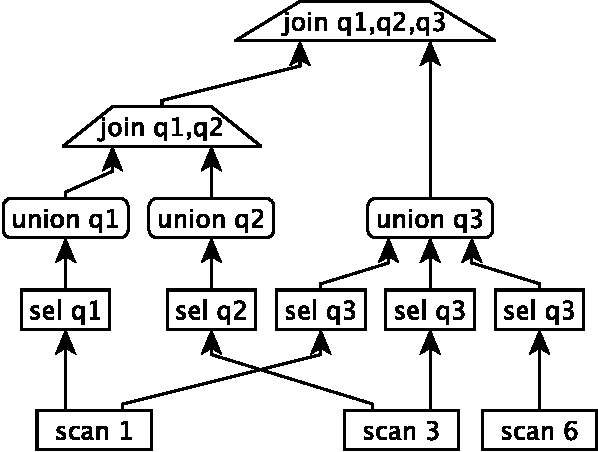
\includegraphics[width=0.6\linewidth]{figs/plan-crop.pdf}
  \caption{Query plan for the example query.}
\label{fig:plan}
\vspace{-0.5cm}
\end{figure}
\begin{example}
  Fig.~\ref{fig:plan} shows an example query plan for the 
  query from Fig.~\ref{fig:query}. There are three source scan
  operators, one for each of the sources \emph{(1) ex:beatles},
  \emph{(3) ex:sgt\_pepper}, and \emph{(6) ex:lucy}. Together with 
  selection and union operators, the source scans form 3 access
  plans for the 3 triple patterns $q_1, q_2$, and $q_3$.  The
  outputs of the access plans are then combined using 2 join operators.

  As the sources \emph{ex:beatles} and \emph{ex:sgt\_pepper} contain
  relevant data for more than one triple pattern ($q_1,q_3$ and
  $q_2,q_3$, respectively), their source scans are shared, i.e. the
  outputs of the these operators feed into 2 access plans.
\end{example}


\subsection{Pareto Optimal Plans} 
Optimality is not clearly defined in the Linked Data context. Traditionally, completeness is assumed such that all results have to be computed. Optimality in this case is defined with respect to processing cost, and optimization techniques aim to find plans that are cost-optimal, i.e. produce all results at lowest cost. As discussed, completeness is not practical in Linked Data query processing and existing approaches (select and) process only a few sources~\cite{harth_data_2010,ladwig_linked_2010}. Not only cost but also the number of results have to be considered here. Further, other criteria such as the trustworthy of sources and the quality of data may play an important role. This results in a \emph{multi-objective} optimization problem. 

For a query $Q$, % = \{t_1, \ldots, t_n\}
the goal is to compute the skyline (Pareto set) of query plans that represents different trade-offs between multiple objectives. For clarity of presentation, we will focus on the two main objectives of maximizing \emph{output cardinality}, $card(\cdot)$, and \emph{processing cost}, $cost(\cdot)$. 
%Further, we define cost as $score(\cdot) = \frac{1}{cost(\cdot)}$ such that the objective is to maximize the score and output cardinality.  \todo{use cost instead of score everywhere}
The skyline of a set of solutions is defined using a \emph{dominance}
relation that relates the multiple objectives. A query plan is considered to dominate another plan, if it is at least as good in all objectives and better in at least one objective:

\begin{definition}[Dominance]
  Given two query plans $p_1$ and $p_2$, $p_1 \mbox{ \textnormal{dominates}
  } p_2$ ($p_1 > p_2$) if both the cost and cardinality of $p_1$ are ``better'' or equal
  to the score and cardinality of $p_2$, and either the score or
  cardinality is strictly ``better'' than the score or cardinality of
  $p_2$, i.e. $cost(p_1) \leq cost(p_2) \wedge card(p_1) \geq
  card(p_2) \wedge ((cost(p_1) < score(p_2) \vee card(p_1) >
  card(p_2)) \Rightarrow p_1 > p_2$.
\end{definition}


\begin{definition}[Pareto Optimal Plans]
  Given a query $Q$ and a set of query plans $P(Q)$ for $Q$, the \emph{Pareto}
  set $P^*(Q) \subseteq P(Q)$ comprises all plans that are not
  dominated by any other plan in $P(Q)$, i.e. $P^*(Q) = \{p_i \in P(Q) | \neg\exists p_j\in P(Q), p_j  > p_i\}$. We denote the set of
  dominated plans as $P^-(Q) = P(Q) \setminus P^*(Q)$. The set of \emph{optimal plans} for $Q$, denoted as $P^+(Q)$, is the Pareto set of plans for $Q$, i.e. $P^+(Q) = P^*(Q)$.
\end{definition}


%%% Local Variables: 
%%% mode: latex
%%% TeX-master: "paper"
%%% End: 
